\documentclass{article}
\usepackage{amsmath}
\usepackage{amssymb}
\usepackage{mathtools}
\usepackage{fullpage}
\usepackage{enumerate}
\usepackage{graphicx}
\newcommand{\tmblank}{\textvisiblespace}
\newcommand*{\<}{\langle}
\renewcommand*{\>}{\rangle}

\title{Computer Science 540 Notes \\ Theory of Computing}
\author{Mendel C. Mayr}
\date{\today}

\begin{document}
	\maketitle
	\begin{center}
		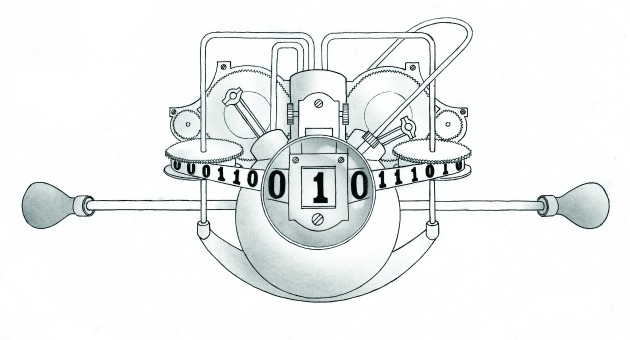
\includegraphics[width = 3.8in]{turingMachine.jpg}
		\end{center}
	\tableofcontents
	\clearpage

	\section{Regular languages}
		\subsection{Finite Autonoma}
			Deterministic finite autonoma consist of a set of states with transitions between states. Includes initial state and end state(s).
			\begin{center}
				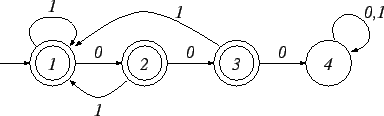
\includegraphics[width = 3.0in]{dfaExample.png} \\
				An example of a deterministic finite automata \\
				\end{center}
			Formal definition: A determinisitic finite automata is a tuple $M = (Q, \Sigma, q_0, F, \delta)$, where: \\
			\begin{enumerate}
				\item $Q = $ finite set of states
				\item $\Sigma = $ finite set of input symbols (called the DFA's alphabet) \\
				$\Sigma^*$ denotes set of all strings that can be made from elements of $\Sigma$ 
				\item $q_0 = $ the initial state, where $q_0 \in Q$ 
				\item $F = $ set of final states, $F \subseteq Q$ 
				\item $\delta = $ a transition function, where $\delta : Q \times \Sigma \to Q$
				\end{enumerate}
			The transition function $\delta$ can be extended to accept strings of symbols: $\hat{\delta} : Q \times \Sigma^*$ \\
			The function $\hat{\delta}$ can be defined by induction: \\
			\\
			Base case: $\hat{\delta}(q, \varepsilon) = q $ where $\varepsilon$ is an empty string \\
			Base case: $\hat{\delta}(q, a) = \delta(q, a) $ where $a \in \Sigma$ \\
			Inductive case: $\hat{\delta}(q, x)$, where $x \in \Sigma^*, a \in \Sigma, x = ay, y \in \Sigma^*, |y| = |x| - 1$
			\begin{equation*}
				\hat{\delta}(q, x) = \hat{\delta}(q, ay) = \hat{\delta}(\delta(q, a), y)
				\end{equation*} 
			\\
			Lemma: $\forall q \in Q$ and $\forall x, y \in \Sigma^*$, $\hat{\delta}(\hat{\delta}(q, x), y) = \hat{\delta}(q, xy)$ \\
			\\
			Provable by induction on $k = |x|$: \\
			Base case $k = 0$, $x = \varepsilon$: $\hat{\delta}(\hat{\delta}(q, \varepsilon), y) = \hat{\delta}(q, y) = \hat{\delta}(q, \varepsilon y)$ \\
			Base case $k = 1$, $x = a \in \Sigma$: $\hat{\delta}(\hat{\delta}(q, a), y) = \hat{\delta}(\delta(q, a), y) = \hat{\delta}(q, ay)$ \\
			Inductive case $|x| = k + 1$, $x = az \text{ for } a \in \Sigma, z \in \Sigma^*, |z| = k$: \\
			\begin{equation*}
				\hat{\delta}(q, azy) = \hat{\delta}(\delta(q, a), zy) = \hat{\delta}(\hat{\delta}(\delta(q, a), z), y) = \hat{\delta}(\hat{\delta}(q, az), y)
				\end{equation*}
			\\
			Since we can describe $\delta$ as simply $\hat{\delta}$ when taking a string of length 1, the extended transition function $\hat{\delta}$ can henceforth be denoted as simply $\delta$ \\
			\\
			The language of (i.e. solutions to) deterministic finite autonoma $M$ is $L(M) = \{x \in \Sigma^* |\: \delta(q_0, x) \in F \}$ \\
			Regular language: a language recognized by some finite automaton. (Note that languages are composed of strings) \\
			\\
			Operations on regular languages (i.e. regular operations):
			\begin{enumerate}[(i)]
				\item Union: $A \cup B = \{x\:|\:x \in A \text{ or } x \in B\}$
				\item Concatenation: $A \circ B = \{xy\:|\:x \in A \text{ and } y \in B\}$
				\item Star: $A* = \{x_1x_2\:...\:x_k\:|\:k \geq 0 \text{ and each } x_i \in A\}$. Note that $\varepsilon \in A$ for any $A$ (i.e. when $k = 0$).
				\end{enumerate}
			Theorem: the class of regular languages is closed under the union operation (i.e. if $A_1$ and $A_2$ are regular languages, so is $A_1 \cup A_2$) \\
			\\
			Proof: let $M_1 = (Q_1, \Sigma, \delta_1, q_1, F_1)$ recognize $A_1$, and $M_2 = (Q_2, \Sigma, \delta_2, q_2, F_2)$ recognize $A_2$ \\
			Then the automaton $M = (Q, \Sigma, \delta, q, F)$ recongizes $A_1 \cup A_2$, where:
			\begin{enumerate}
				\item $Q = Q_1 \times Q_2 = \{(r_1, r_2)\:|\:r_1 \in Q_1 \text{ and } r_2 \in Q_2\}$
				\item $\Sigma$ unchanged in the case of identical alphabets
				\item $\delta((r_1, r_2), a) = (\delta_1(r_1, a), \delta_2(r_2, a))$
				\item $q = (q_1, q_2)$
				\item $F = \{(r_1, r_2)\:|\:r_1 \in F_1 \text{ or } r_2 \in F_2\}$
				\end{enumerate}
		\subsection{Nondeterminism}
			\begin{center}
				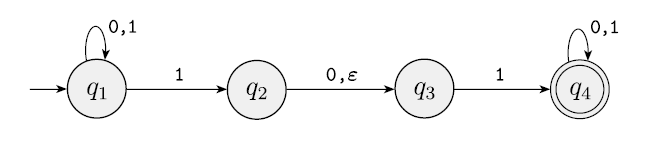
\includegraphics[width = 3.0in]{nfa.png} \\
				An example of a nondeterministic finite automata \\
				\end{center}
			Differences between deterministic finite automata (DFA) and nondeterministic finite automata (NFA):
			\begin{enumerate}[(i)]
				\item States in an NFA can have any non-negative number of exiting transitions for each alphabet symbol
				\item Symbols for transition can include members of the alphabet or the label $\varepsilon$
				\end{enumerate}
			Formal definition: A nondeterminisitic finite automata is a tuple $M = (Q, \Sigma, q_0, F, \delta)$, where:
			\begin{enumerate}[(i)]
				\item $Q = $ finite set of states
				\item $\Sigma = $ alphabet of symbols \\
				$\Sigma^*$ denotes set of all strings that can be made from elements of $\Sigma$ 
				\item $q_0 = $ the initial state, where $q_0 \in Q$ 
				\item $F = $ set of final states, $F \subseteq Q$ 
				\item $\delta = $ a transition function, where $\delta : Q \times \Sigma \to \mathcal{P}(Q)$
				\end{enumerate}
			$\delta$ for an NFA can be extended. $\hat{\delta} : Q \times \Sigma^*$ is defined inductively\\
			Base case: $\hat{\delta}(q, \varepsilon) = {q}$ \\
			Base case: $\hat{\delta}(q, a) = \delta(q, a)$ where $a \in \Sigma$ \\
			Inductive case: $\hat{\delta}(q, wa) = \bigcup\limits_{p \in \hat{\delta}(q, w)}\delta(p, a)$ \\
			\\
			$\hat{\delta}$ can also be defined to accept subsets of $Q$ \\
			$\hat{\delta}(P, w) = \bigcup\limits_{p \in P}\hat{\delta}(p, w)$, where $P \subseteq Q$, $w \in \Sigma^*$ \\
			Corrolary: $\hat{\delta}(q, xy) = \hat{\delta}(\hat{\delta}(q, x), y)$ \\
			\\
			The language accepted by the NFA is $L(A) = {x \in \Sigma^*\:|\:\hat{\delta}(q, x) \cap F \neq \emptyset}$ \\
			\\
			Computation with an NFA: when at a state with multiple exist transitions for the same symbol, the NFA produces copies and follows all transitions for that symbol in parallel. Each copy proceeds the read the string non-deterministically. If a symbol doesn't appear at a state, that copy of the NFA dies. If any branch ends at an accept state, the NFA accepts the input string. At a state with the $\varepsilon$ exit transtion, copies of the NFA follow the $\varepsilon$ transitions, while one copy remains in the current state. \\
			\\
			NFAs and DFAs are recognize the same class of languages, despite the NFAs notational superiority. Two machines are said to be equivalent if they recognize the same language. Note that nondeterministic finite automata are generalizations of deterministic finite automata (i.e. all DFAs are NFAs). Furthermore, all NFAs can be converted into DFAs (although the NFA may offer a much simpler representation.) \\
			\\
			Theorem: every NFA can be represented by an equivalent DFA \\
			Let $N = (Q, \Sigma, \delta_N, q_0, F_N)$ be the NFA that recongizes language $A$, then an equivalent DFA would be $M = \mathcal{P}(Q), \Sigma, \delta_M, \{q_0\}, F_M)$, where $F_M = \{S \subseteq Q | S \cap F \neq \emptyset\}$, and $\delta_M$ is, for all $S \in \mathcal{P}(Q), a \in \Sigma$, defined as \\
			\begin{equation*}
				\delta_M(S, a) = \hat{\delta}_N(S, a) = \bigcup\limits_{s \in S}\delta_M(s, a)
				\end{equation*}
			Corrolary: a language is regular if and only if it is recognized by some nondeterministic finite automata \\
			\\
			Using NFAs, proofs can be constructed for the closure of the regular operations \\
			\\
			Theorem: class of regular languages is closed under concatenation \\
			Let NFAs $N_1 = (Q_1, \Sigma, \delta_1, q_1, F_1)$ recognize $A_1$ and $N_2 = (Q_2, \Sigma, \delta_2, q_2, F_2)$ recognize $A_2$ \\
			The NFA $N = (Q, \Sigma, \delta, q_1, F_2)$ recongizes $A_1 \circ A_2$, where $Q = Q_1 \cup Q_2$ \\
			The transition function $\delta$ is defined so that the final states of $N_1$ transitions via $\varepsilon$ to the intial state of $N_2$, i.e. $\delta$ is, for $q \in Q$ and $a \in \Sigma_\varepsilon$ defined as
			\begin{enumerate}[(i)]
				\item $\delta(q, a) = \delta_1(q, a)$ when $q \in Q_1$ and $q \notin F_1$
				\item $\delta(q, a) = \delta_1(q, a)$ when $q \in F_1$ and $a \neq \varepsilon$
				\item $\delta(q, a) = \delta_1(q, a) \cup {q_2}$ when $q \in F_1$ and $a = \varepsilon$
				\item $\delta(q, a) = \delta_2(q, a)$ when $q \in Q_2$
				\end{enumerate}
			Theorem: class of regular languages closed under the star operation
			Let $N_1 = (Q_1, \Sigma, \delta_1, q_1, F_1)$ recognize $A_1$, then $N = (Q, \Sigma, \delta, q_0, F)$ recognizes $A_1^*$. N includes a new initial state that transitions via $\varepsilon$ to $q_1$, and $q \in F$ transition via $\varepsilon$ to $q_1$. So $Q = {q_0} \cup Q_1$, $q_0$ is the new initial state, $F = {q_0} \cup F_1$, and $\delta(q, a)$ is defined normally, except in cases
			\begin{enumerate}[(i)]
				\item $\delta(q \in F_1, a = \varepsilon) = \delta_1(q, a) \cup {q}$
				\item $\delta(q_0, a = \varepsilon) = {q_1}$
				\item $\delta(q_0, a \neq \varepsilon) = \emptyset$
				\end{enumerate}
		\subsection{Regular expressions}
			Regular expressions are built from regular operations acting on languages \\
			Formal (inductive) definition of regular expression (with assocated languages): $R$ is a regular expression if $R = $
			\begin{enumerate}[(i)]
				\item $a$ for some $a \in \Sigma$, $L(a) = {a}$
				\item $\varepsilon$, $L(\varepsilon) = {\varepsilon}$
				\item $\emptyset$, $L(\emptyset) = \emptyset$
				\item $R_1 \cup R_2$, where $R_1, R_2$ are regular expressions, $L(R_1 \cup R_2) = L(R_1) \cup L(R_2)$
				\item $R_1 \circ R_2$ where $R_1, R_2$ are regular expressions, $L(R_1 \circ R_2) = L(R_1) \times L(R_2)$
				\item $R_1^*$, where $R_1$ is a regular expression, $L(R_1^*) = L(R_1)^*$
				\end{enumerate}
			Order of regular operations: star, concatenation, union \\
			\\
			Note the identities:
			\begin{enumerate}[(i)]
				\item for $\omega \in \Sigma$, $\omega \circ \varepsilon = \omega$
				\item $R \cup \emptyset = R$
				\item $R \circ \varepsilon = R$
				\end{enumerate}
			Fact: regular expressions are equivalent if their languages are the same
			\\
			Notation for regular expresions:
			\begin{enumerate}[(i)]
				\item $R^+ = RR*$, all contatenations of strings from $R$ excluding the possibility of 0 strings (i.e. excludes $\varepsilon$)
				\item $R^k =$ concatenation of $k$ $R$s with each other
				\item $L(R) =$ the language described by regular expression $R$ 
				\end{enumerate}
			Theorem: a language is regular if and only if some regular expression describes it \\
			\\
			Lemma: if a regular expression describes a language, then it is regular \\
			NFAs can be constructed for each possibility that counts as a regular expression
			\begin{enumerate}[(i)]
				\item $R = a$, so $L(R) = \{a\}$ and $N = (\{q_1, q_2\}, \Sigma, \delta, q_1, \{q_2\})$, $\delta(q_1, a) = \{q_2\}$ and $\delta(r, b) = \emptyset$ for $r \neq q_1$ or $b \neq a$
				\item $R = \varepsilon$, so $L(R) = \{\varepsilon\}$ and $N = (\{q_1\}, \Sigma, \delta, q_1, \{q_1\})$, $\delta(r, b) = \emptyset$ for any $r$ and $b$
				\item $R = \emptyset$, so $L(R) = \{\emptyset\}$ and $N = (\{q\}, \Sigma, \delta, q, \emptyset)$, $\delta(r, b) = \emptyset$ for any $r$ and $b$
				\item For the last 3 cases, we can use the NFAs constructed iofn proving the closure of the regular operations
				\end{enumerate}
			Note that these formalizations can guide the construction of NFAs for any regular expression \\
			\\
			Lemma: if a language is regular, then it is described by a regular expression \\
			Requires the concept of a generalized nondeterministic finite automaton (GNFA) \\
			GNFAs are nondeterministic finite autonoma, except the state transitions can be labeled with regular expressions instead of only members of $\Sigma \cup \{\varepsilon\}$ \\
			For simplicity, assume for the GNFA that
			\begin{enumerate}[(i)]
				\item Start state has transitions to every other state but no transitions to it from other states
				\item There is only one accept state, different from the start state, that has transitions from all other states but none leaving it to any other states
				\item Except for the initial and final states, one transition goes from every state to every other state and from each state to itself
				\end{enumerate}
			To convert a DFA to an equivalent GNFA, add a new start state with $\varepsilon$ transitions to old start state and add a new accept state with $\varepsilon$ transitions from old accept states. Arrows with multiple labels (or multiple arrows in the same direction between two states) can be replaced with transitions labeled by the union of the old labels. Missing transitions can be filled by adding $\emptyset$-labled transitions \\
			\\
			Every GNFA with $k > 2$ states can be reduced to a GNFA with $k - 1$ states until there are only $k = 2$ states (i.e. the start and accept states), in which case the regular expression labels the transition between them \\
			\\
			To reduce a GNFA, remove a non-start, non-accept state denoted $q_{rip}$, and replace transitions between state $q_i$ and $q_j$ with a regular expression describing all strings that would either transition the machine directy from $q_i$ to $q_j$ or between the states via $q_{rip}$ \\
			\\
			In a simpler sense, if in the old machine $R_1: q_i \to q_{rip}, R_2: q_{rip} \to q_{rip}, R_3: q_{rip} \to q_j, R_4: q_i \to q_j$, then the transition from $q_i$ to $q_j$ gets the new label $(R_1)(R_2)*(R_3) \cup (R_4)$ \\
			\\
			Formal definition of generalized nondeterministic finite automaton: $(Q, \Sigma, \delta, q_{start}, q_{accept})$ where
			\begin{equation}
				\delta : (Q - \{q_{accept}\}) \times (Q - \{q_{start}\}) \to \mathcal{R}
				\end{equation}
			(Finally) concluding the proof of the lemma and theorem, the regular expression can be simply derived by converting the corresponding DFA to a GNFA and reducing to a regular expression
		\subsection{Nonregular languages}
			Pumping lemma: if $A$ is a regular language, then there exists a number $p$ (the pumping length) where if $s$ is any string in $A$ of length at least $p$, then $s$ may be divided into three pieces, $s = xyz$ such that:
			\begin{enumerate}[(i)]
				\item for each $i \geq 0$, $xy^iz \in A$
				\item $|y| > 0$, and
				\item $|xy| \leq p$
				\end{enumerate}
			Let $M = (Q, \Sigma, \delta, q_1, F)$ be a DFA recognizing $A$ and $p$ be the number of states of $M$. \\
			Let $s = s_1s_2...s_n$ be a string in $A$ of length $n$, where $n \geq p$ \\
			Let $r_1,\:...\:, r_{n + 1}$ be the sequence of states when processing $s$, so $r_{n + 1} = \delta(r_i, s_i)$ for $1 \leq i \leq n$ \\
			\\
			Since there are $p$ states in $M$ and the string $s$ is of length $n \geq p$, at least one of the states in $r_1,\:...\:, r_{n + 1}$ must be repeated at least once according to the pigeonhole principle \\
			Let the state at the first instance be $r_j$ and the state upon the first repetition be $r_l$ \\
			Now let $x = s_1...s_{j - 1}, y = s_j...s_{l - 1}, z = s_l...s_n$, which satisfies the properties \\
			\\
			To prove that a language $B$ is not regular, assume its regularity. Then find a string $s$ in the $B$ with length $p$ or greater that cannot be pumped. Then demonstrate that all ways of dividing $s$ into $x, y, z$ yields an instance $i$ in which $xy^iz \notin B$. This demonstrates that $B$ is not regular \\
			\\
			Note that satisfying the pumping property is a neccesary but not sufficient property of regular languages
		\subsection{Myhill-Nerode theorem}
			Suppose: $(\delta(q_0, x) = \delta(q_0, y)) \to (xz \in L) \iff (yz \in L)$ for all $z \in \Sigma^*$ \\
			Let $M$ be a DFA, then two strings $x$ and $y$ are equivalent via the equivalence relation $x \equiv_M y$ if and only if $\delta(q_0, x) = \delta(q_0, y)$. Then strings $x$ and $y$ are said to be in the same equivalence class \\
			\\
			Each state of the DFA $M$ corresponds to an equivalence class, each of which forms part of $\Sigma^*$, and transitions in $M$ map to transitions between equivalence classes \\
			\\
			Given $L \subseteq \Sigma^*$, define $\equiv_L$ where $(x \equiv_L y) \iff (\forall z \in \Sigma^*(xz \in L \iff yz \in L))$ \\
			\\
			Theorem: the following are equivalent
			\begin{enumerate}[(1)]
				\item L is a regular set
				\item L is the union of equivalence classes of an equivalence relation that is right invariant and of finite index \\
				Right invariant: $XR_My \to \forall z (xz)R_M(yz)$ \\
				Finite index: finite number of equivalence classes
				\item $\equiv_L$ otherwise denoted $R_L$, is of finite index
				\end{enumerate}
			Proof: (1) $\to$ (2) \\
			$L = L(M)$ for some DFA $M$, define the equivalence relation $R_M$ \\
			Right invariance due to nature of DFA transitions \\
			By definition: equivlence classes in 1-to-1 relation with DFA states \\
			Taking the union of classes corresponding to reachable final states \\
			\\
			Proof: (2) $\to$ (3) \\
			If $xR_My \to xR_Ly$, then $\#R_L \leq \#R_M \geq \infty$, where $\#R$ is the number of equivalence classes in relation $R$ \\
			Derivable from definitions: $xz \in L \iff yz \in L$ \\
			\\
			Proof: (3) $\to$ (1) \\
			We can build a DFA out of the equivalence classes of $R_L$ \\
			By the definition of $R_L$, since $xR_Ly \to (xzw \in L \iff yzw \in L)$, $R_L$ is right invariant \\
			We define DFA $M = (Q, \Sigma, \delta, q_0, F)$, where
			\begin{enumerate}[(i)]
				\item $Q$ is the set of equivalence classes of $R_L$
				\item $q_0 = [\varepsilon]$, the equivalence class contatining $\varepsilon$
				\item $\delta([x], a) = [xa]$
				\item $F = \{[x]\:|\:x \in L\}$
				\end{enumerate}
		\clearpage

	\section{Context-free languages}
		\subsection{Context-free grammars}
			Formal definition of context-free grammar (CFG): \\
			A context-free grammer is a 4-tuple $(V, \Sigma, R, S)$, where
			\begin{enumerate}
				\item $V$ is a finite set called the variables
				\item $\Sigma$ is a finite set, disjoint from $V$, called the terminals
				\item $R$ is a finite set of rules, where $R \subseteq \{(v, w)\}$ where $v \in V, w \in (V \cup \Sigma)^*$
				\item $S \in V$ is the start variable
				\end{enumerate}
			Notation: variables denoted by captial letters, terminals and strings denoted with lowercase \\
			\\
			For $v \in V$, $a, b, c \in (V \cup \Sigma)^*$:
			\begin{enumerate}
				\item Suppose $v \to b$ is a rule
				\item $avc$ is said to yield $abc$, denoted $avc \Rightarrow abc$
				\item $a$ derives $b$ if $u = v$ or there exists $a_1, a_2,\:...\:, a_k$ for $k \geq 0$ such that
				\begin{equation*}
					a \Rightarrow a_1 \Rightarrow a_2 \Rightarrow\:...\:\Rightarrow a_k \Rightarrow b
					\end{equation*}
				\item Language of the grammar is $\{w \in \Sigma^*\:|\:S \Rightarrow^* w\}$
				\end{enumerate}
			Fact: any DFA can be converted into an equivalent CFG
			\begin{enumerate}
				\item Variable $R_i$ for each state $q_i$
				\item Rule $R_i \to aR_j$ if $\delta(q_i, a) = q_j$
				\item Rule $R_i \to \varepsilon$ if $q_i$ is accept state
				\end{enumerate}
			If a grammar generates the same string in multiple ways, the string is derived ambiguously from the grammar \\
			Leftmost derivation: at every step, the leftmost remaining variable is the one replaced \\
			Formally, a string $w$ is derived ambiguously in context-free grammar $G$ if it has two or more leftmost derivations. Grammar $G$ is ambiguous if it generates some string ambiguously \\
			Inherently ambiguous languages can only be generated by ambiguous grammars \\
			\\
			Chomsky normal form: a context-free grammar is in Chomsky normal form if every rule is of the form $A \to BC$ or $A \to a$ where $a \in \Sigma$, $A, B, C \in \Sigma$, $B$ nor $C$ is the start variable. The rule $S \to \varepsilon$ also permitted \\
			Theorem: any context-free language is generated by a context-free grammar in Chomsky normal form 
			\begin{enumerate}
				\item Define new start variable $S_0$ and rule $S_0 \to S$ where $S$ is original start variable
				\item Eliminate all $\varepsilon$ rules: \\
				For $A \neq S_0$, eliminate $A \to \varepsilon$ \\
				Replace rules of form $R \to uAv$ (where $u, v \in \{\Sigma \cup V\}^*$) with rules $R \to uv$ \\
				Replacement done for each occurence of an $A$ (e.g. removing $R \to uAvAw$ adds $R \to uAvw, \\
				R \to uvAw, R \to uvw$) \\
				Replace $R \to A$ with $R \to \varepsilon$ unless $R \to \varepsilon$ had been previously removed
				\item Handle unit rules: \\
				Eliminate unit rule of form $A \to B$ \\
				Whenever rule of form $B \to u$ appears, add rule $A \to u$ unless $A \to u$ previously removed \\
				Repeat steps until unit rules eliminated
				\item Convert remaining rules into proper form : \\
				Eliminate rules of form $A \to u_1u_2...u_k$ where $k \geq 3$ and each $u_i$ is a variable or terminal symbol \\
				Replace with rules: $A \to u_1A_1, A_1 \to u_2A_2,\:...\:, A_{k - 2} \to u_{k - 1}u_k$ \\
				Replace any terminal $u_i$ in preceding rule(s) with new variable $U_i$ and add rule $U_i \to u_i$
				\end{enumerate}
			Consider the grammar that generates, unambiguously and with left associativity, mathematical expressions with $i$, $+$, $*$, $($, and $)$ 
			\begin{enumerate}[(i)]
				\item $E \to E + T | T$
				\item $T \to T * F | F$
				\item $F \to (E) | i$
				\end{enumerate}
			Proof of non-ambiguity: intuitive ideas \\
			If $D$ be the condition $E \Rightarrow x$ or $T \Rightarrow x$ or $F \Rightarrow x$, then:
			\begin{enumerate}[(i)]
				\item If $D$, then $|x| \geq 1$
				\item If $D$ and $|x| = 1$, then $x = i$ (and vice versa)
				\item If $D$, then $+$ or $*$ cannot appear at beginning or end of $x$
				\end{enumerate}
			Lemma: If $E \Rightarrow x$, then $N_((x) = N_)(x)$, and for all prefixes $y$ of $x$, $N_((y) \geq N_)(y)$ \\
			If $T \Rightarrow x$, then $N_((x) = N_)(x)$, and for all prefixes $y$ of $x$, $N_((y) \geq N_)(y)$ \\
			If, in the statement above, $x = y + z$, then $N_((y) > N_)(y)$ \\
			If $F \Rightarrow x$, then $N_((x) = N_)(x)$, and if $y \neq \varepsilon$ and $y$ is a proper prefix (prefix not-equal-to) of $x$, then $N_((y) > N_)(y)$ \\
			\\
			Now to prove by induction on the number of steps in a derivation: 
			\begin{enumerate}
				\item Case: $E \xRightarrow{i} x$, then $E \Rightarrow T \xRightarrow{i - 1} x$ or \\
				$E \Rightarrow E + T \Rightarrow y + z = x$, and $E \Rightarrow y, T \Rightarrow z$ in less than $i$ steps
				\item Case: $T \xRightarrow{i} x$, then $T \Rightarrow F \xRightarrow{i - 1} x$ or \\
				$T \Rightarrow T * F \Rightarrow y' * z' = x$, conditions $T$ derivation of lemma satisfied 
				\item Case: $F \xRightarrow{i} x$, $T \Rightarrow (E) \Rightarrow (y) = x$, conditions satisfied
			\end{enumerate}
			Theorem: this grammar is non-ambiguous \\
			Let $F \xRightarrow{i} x$, if $|x| = 1$, unique derivation for $F \Rightarrow i$ \\
			Now let $|x| > 1$: the first step must be $F \to (E) \xRightarrow{i - 1} (y) = x$, and $E \Rightarrow{i - 1} y$ \\
			Let $T \xRightarrow{i} x$ and $|x| > 1$, suppose that there are two derivations from $T \Rightarrow T * F$ \\
			Let $y_1 * z_1$ and $y_2 * z_2$ be the two derivations, by contradiction using conditions, this is not possible
		\subsection{Pushdown automata}
			Pushdown automata (PDAs): NFAs extended with stacks equivalent in power to context-free grammars \\
			Recall that $\Sigma_\varepsilon = \Sigma \cup \{\varepsilon\}$ and $\Gamma_\varepsilon = \Gamma \cup \{\varepsilon\}$, thus a pushdoseteqwn autonoma is a 6 tuple $(Q, \Sigma, \Gamma, \delta, q_0, F)$ where 
			\begin{enumerate}[(i)]
				\item $Q$ is the set of states
				\item $\Sigma$ is the input alphabet
				\item $\Gamma$ is the stack alphabet
				\item $\delta: Q \times \Sigma_\varepsilon \times \Gamma_\varepsilon \to \mathcal{P}(Q \times \Gamma_\varepsilon)$ is the transition function
				\item $q_0 \in Q$ is the start state
				\item $F \subseteq Q$ is the set of accept states
				\end{enumerate}
			A pushdown automaton $M = (Q, \Sigma, \Gamma, \delta, q_0, F)$ computes as follows. It accepts input $w = w_1w_2...w_m$ where $w_i \in \Sigma_\varepsilon$ and sequence of states $r_0, r_1,\:...\:, r_m \in Q$ and strings $s_0, s_1,\:...\:, s_m \in \Gamma^*$ exist that satisfy the following conditions: the strings $s_i$ represent the sequence of stack contents that $M$ has on the accepting branch of computation
			\begin{enumerate}[(i)]
				\item $r_0 = q_0$ and $s_0 = \varepsilon$, i.e. $M$ starts out properly, in the start state and with an empty stack
				\item For $i = 0,\:...\:, m - 1$, we have $(r_{i + 1}, b) \in \delta(r_i, w_{i + 1}, a)$, where $s_i = at$ and $s_{i + 1} = bt$ for some $a, b \in \Gamma_\varepsilon$ and $t \in \Gamma^*$, i.e. $M$ moves properly according to the state, stack, and next input symbol
				\item $r_m \in F$, i.e. the accept state occurs at input end
				\end{enumerate}
			Transition interpretation of $a, b \to c$: when reading $a$ from input, replace symbol $b$ on top of stack with $c$. If $a$ is $\varepsilon$, transition can be made without reading input. If $b$ is $\varepsilon$, no symbol needs to be popped. If $c$ is $\varepsilon$, no symbol is pushed. \\
			i.e. transition label is of form $inputSymbol, popped \to pushed$ \\
			\\
			Transition notation: $\delta($state, input, pop$)$ = $\{(\text{next state, push})\:...(\text{next state, push})\}$
			\\
			Equivalence with context-free grammars: \\
			Theorem: a language is context-free if and only if some pushdown automaton recongizes it \\
			\\
			Lemma: if a language is context-free, some pushdown automaton recognizes it \\
			Proof idea: a pushdown automaton that recognizes a context-free language operates as such:
			\begin{enumerate}[(i)]
				\item Put the marker symbol $\$$ and the start variable on the stack
				\item Repeat the following steps:
				\begin{enumerate}[(a)]
					\item If the top of the stack is variable $A$, nondeterministically select rules for $A$ and substitute $A$ with whatever $A$ yields
					\item If the top of the stack is terminal $a$, read the next symbol of the input. If they don't match, reject this branch of the computation
					\item If the top of the stack is the symbol $\$$, go to accept state
					\end{enumerate}
				\end{enumerate}
			Proof: define a pushdown automaton $P = (Q, \Sigma, \Gamma, \delta, q_{start}, F)$ defining a CFL \\
			\\
			Let $q$ and $r$ be states of $P$ and let $a \in \Sigma_\varepsilon$ and $s \in \Gamma_\varepsilon$. The PDA should transition from $q$ to $r$ when reading $a$ and popping $s$. It should also push the entire string $u = u_1...u_l$ to the stack at the same time. \\
			Implement by introducting new states $q_1,\:...\:, q_{l - 1}$ and defining the $\delta$ as such:
			\begin{itemize}
				\item[--] $(q_1, u_l) \in \delta(q, a, s)$
				\item[--] $\delta(q_1, \varepsilon, \varepsilon) = \{(q_2, u_{l - 1})\}$
				\item[--] $\delta(q_2, \varepsilon, \varepsilon) = \{(q_3, u_{l - 2})\}$ \\
				...
				\item[--] $\delta(q_{l - 1}, \varepsilon, \varepsilon) = \{(r, u_1)\}$
				\end{itemize}
			The states of $P$ are $Q = \{q_{start}, q_{loop}, q_{accept}\} \cup E$ where $E$ is the set of states needed as above \\
			\\
			The transition function is defined as such (analog in previous proof idea): 
			\begin{enumerate}[(i)]
				\item $\delta(q_{start}, \varepsilon, \varepsilon) = \{q_{loop} S\$\}$ i.e. stack intitialized to contain symbol $\$$ and start variable $S$
				\item Main loop for second step:
				\begin{enumerate}[(a)]
					\item $\delta(q_{loop}, \varepsilon, A) = \{(q_{loop}, w)\:|\:(A \to w) \in R\}$
					\item $\delta(q_{loop}, a, a) = \{(q_{loop}, \varepsilon)\}$
					\item $\delta(q_{loop}, \varepsilon, \$) = \{(q_{accept}, \varepsilon\}$ 
					\end{enumerate}
				\end{enumerate}
			Thus concludes the forward direction of the CFL/PDA-equvialence theorem \\
			\\
			Lemma: if a pushdown automaton recongizes a language, then the language is context free \\
			Preliminaries: every pushdown automaton $P$ can be modifed to have 3 features
			\begin{enumerate}[(i)]
				\item Has single accept state $q_{accept}$
				\item Empties stack before accepting
				\item Each transition pushes or pops, but not both at the same time
				\end{enumerate}
			Proof: let pushdown automaton $P = (Q, \Sigma, \Gamma, \delta, q_0, \{q_{accept}\})$ and construct $G$ \\
			The variables of $G$ are $\{A_{pq} | p, q \in Q\}$, with start variable being $A_{q_0, q_{accept}}$ \\
			The rules of $G$ can be described as such:
			\begin{enumerate}
				\item For each $p, q, r, s \in Q$, $u \in \Gamma$, and $a, b \in \Sigma_\varepsilon$, if $\delta(p, q, \varepsilon)$ contains $(r, u)$ and $\delta(s, b, u)$ contains $(r, u)$ and $\delta(s, b)$ contains $(q, \varepsilon)$, put rule $A_{pq} \to aA_{rs}b$ in $G$
				\item For each $p, q, r \in Q$, put rule $A_{pq} \to A_{pr}A{rq}$ in $G$
				\item For each $p \in Q$, put rule $A_{pp} \to \varepsilon$ in $G$
				\end{enumerate}
			To prove this construction works requires that $A_pq$ generates $x$ if and only if $x$ brings $P$ from $p$ with an empty stack to $q$ with an empty stack. Both directions provable by induction (not shown here) 
		\subsection{Non-context-free languages}
			Pumping lemma for context-free languages: if $A$ is a context-free language, then there exists a number $p$ (the pumping length), where if $s$ is any string in $A$ of length at least $p$, then $s$ may be divided into five pieces $s = uvxyz$ where:
			\begin{enumerate}
				\item for each $i \geq 0$, $uv^ixy^iz \in A$
				\item $|vy| > 0$
				\item $|vxy| \leq p$
				\end{enumerate}
			Proof: let $G$ be a CFG for CLF $A$. Let $b$ be the maximum number of symbols in the right-hand side of a rule (assuming at least 2). Then any node in the parse tree can have at most $b$ children. \\
			Therefore, if the height of a parse tree is at most $h$, the length of the string is at most $b^h$. Conversely, a string with length at least $b^h + 1$ must have a parse tree with height at least $h + 1$ \\
			\\
			Say $|V|$ is the number of variables in $G$. The set the pumping length $p = b^{|V| + 1}$. A string $s \in A$ with length $p$ or more has parse tree at least $|V| + 1$ high \\
			\\
			Let $\tau$ be a parse tree of $s$. The longest path on $\tau$ is at least $|V| + 2$ nodes long, with at most one at the terminal (i.e. $|V| + 1$ variables). By the pigeonhole principle, some variable $R$ is repeated on the path \\
			\\
			Recall the partition $s = uvxyz$. The earlier occurence of $R$ creates string $vxy$, and the later occurence creates string $x$. Repeatedly replacing $x$ with $vxy$ gives the string $uv^ixy^iz$ where $i > 1$, thus satisfying condition 1 \\
			Condition 2 can be satisfied by choosing, for a string $s$, the parse tree $\tau$ with the smallest number of nodes. \\
			Condition 3: since $p = b^{|V| + 1}$, and the height of the parse tree is at least $|V| + 1$, then $|s| \leq b^{|V| + 1} \leq p$ \\
			\\
			As with the pumping lemma for regular languages, the contrapositive of this pumping lemma is used to demonstrate that a language is not context-free
		\clearpage
	
	\section{Church-Turing thesis}
		\subsection{Turing machines}
			$A$ is an axiom system, then a proof of statement $\phi$ is $A \vdash \phi$ \\
			Consistency: void of internal contradiction, i.e. $\neg((A \vdash \phi) \land (A \vdash \neg\phi))$ \\
			Completeness: to demonstrate every true statement, i.e. $\forall\phi((A \vdash \phi) \lor (A \vdash \neg\phi))$ \\
			\\
			Turing machine: requirements
			\begin{enumerate}[(i)]
				\item Simplicity: obvious that what a Turing machine can do is computable
				\item Universality: emcompasses all computable processes
				\end{enumerate}
			Initial configuration of Turing machine: intuitive definitions 
			\begin{enumerate}[(i)]
				\item Start with a infinite sequence of symbols on a fixed alphabet, plus the blank symbol $B$ 
				\item Sequence is composed of a single block of alphabet symbols, bounded by an infinite sequence of blanks 
				\item A finite control unit (has finite states) starts by reading the first symbol
				\item Can proceed both backward and forward, and the unit is able to read and write to the sequence
				\end{enumerate}
			Formal definition is a Turing machine: a Turing machine is a tuple $M = (Q, \Sigma, \Gamma, \delta, q_0, q_{acc}, q_{rej})$
			\begin{enumerate}[(i)]
				\item $Q$ is a finite set of states
				\item $\Sigma$ is the set of input symbols, including the special blank symbol $B$
				\item $\Gamma$ is the set of read-write symbols, so $\Sigma \subset \Gamma$
				\item $\delta$ is a transition function 
				\item $q_0$ is the initial state, $q_{acc}$ is accepting state, $q_{rej}$ is rejecting state
				\end{enumerate}
			The partial function $\delta$ is defined as $\delta: Q \times \Gamma \to Q \times \Gamma \times \{L, R\}$ \\
			\\
			Halting: it is possible for a automaton to reject, either by entering reject state or by never halting. \\
			Note then, that the accepting and rejecting states are not symmetric \\
			We can simply map the rejecting state to another branch of computation \\
			Therefore, without loss of generality: accepting by halting in finite number of steps, or not halt
			\\
			Notation: a configuration of a Turing machine is written as $uqv$ where $u$ and $v$ are strings written on the tape, $q$ is the current state, and the control unit is overthe first symbol in $v$ \\
			Configuration $C_1$ yields $C_2$ if the Turing machine can legally go from $C_1$ to $C_2$ in one step \\
			The start configuration of $M$ on input $w$ is $q_0w$ \\
			\\
			A language is Turing-recognizable if some Turing machine accepts it \\
			A language is Turing-recognizable if some Turing machine decides it (i.e. the machine will halt) \\
			\\
			Primitive recursive function: if $g$ and $h$ are primitive recursive functions, define a new $f$, a $(n + 1)$-ary function \\
			$f(x_1, x_2,\:...\:, x_n, 0) = g(x_1, x_2,\:...\:, x_n)$ and \\
			$f(x_1, x_2,\:...\:, x_n, y + 1) = h(x_1, x_2,\:...\:, x_n, y, f(x_1, x_2,\:...\:, x_n, y))$
		\subsection{Variants of Turing machines}
			The Turing machine concept is robust. Variants of Turing machine still recognize the same class of languages \\
			\\
			Multitape Turing machines: \\
			Input on tape 1, all others blank. Reading, writing, and moving some or all of the tapes simultaneously. \\
			Transition function: $\delta: Q \times \Gamma^k \to Q \times \Gamma^k \{L, R, S\}^k$ \\
			Theorem: every multitape Turing machine $M$ has an equivalent single-tape Turing machine $S$ \\
			Proof: let M have $k$ tapes. $S$ tracks contents on a single tape by using a special $\#$ symbol as a delimiter, separating the contents of the different tapes. The location of the heads is denoted by marking the corresponding symbol with a dot. Turing machine $S$ operates as such:
			\begin{enumerate}[(i)]
				\item $S$ starts by representing all $k$ tapes of $M$ \\
				$\#\dot{w_1}w_2\:...\:w_n\#\dot{\tmblank}\#\dot{\tmblank}\#\:...\:\#$
				\item To simulate a single move, $S$ scans the tape from the first $\#$ to the $(k+ 1)$st $\#$ to determine the symbols under the heads. Then $S$ makes a second pass to update the tapes according to the $M$ transition function
				\item If $S$ moves a virtual head on a $\#$, it writes a blank to the cell and shifts all the symbols to accomodate
				\end{enumerate}
			Corollary: a language is Turing-recognizable if and only if some multitape Turing machine recognizes it \\
			\\
			Nondeterministic Turing machines: machine can proceed to multiple possibilities \\
			Transition function: $\delta: Q \times \Gamma \to \mathcal{P}(Q \times \Gamma \times {L, R})$ \\
			Theorem: every nondeterministic Turing machine $N$ has an equivalent deterministic Turing machine $D$ \\
			Proof idea: consider $N$s computation as a tree with the starting configuration at the root. To avoid getting stuck in infinite loops, $D$ visits using breadth-first search. $D$ will accept if it encounters an accepting configuration \\
			\\
			Proof: $D$ has three tapes. Tape 1 is constant and contains the input string. Tape 2 has a copy of $N's$ tape on some computation branch. Tape 3 tracks $D$'s location in the nondeterministic computation tree \\
			\\
			Let $b$ be the maximum branching factor for $N$. The alphabet of Tape 3 is $\Gamma_n = \{1, 2,\:...\:, b\}$. Tape 3 stores a string $a$ representing a node. It means the $a_1$th branch was taken from the root, the $a_2$th branch taken after that, etc. An invalid address designates that such an address cannot be reached \\
			That given, $D$ is described as such:
			\begin{enumerate}[(i)]
				\item Tape 1 contains input $w$ and tapes 2 and 3 are empty
				\item Copy tape 1 to tape 2 and tape 3 is initializaed to $\varepsilon$
				\item Use tape 2 to simulate. Before each step, use the next symbolon tape 3 to determine branch. \\
				Accept or reject if at such a configuration. If no more symbols or invalid address, skips to stage (iv)
				\item Replace string on tape 3 with next string in string ordering, then return to state (ii)
				\end{enumerate}
			Corollary: a language is Turing-recognizable if and only if some nondeterministic Turing machine recognizes it \\
			Corollary: a language is decidable if and only if some nondeterminstic Turing machine decides it \\
			\\
			Enumerator: informally, a Turing machine with an attached printer \\
			An enumerator $E$ starts with a blank input on work tape. The language enumerate by $E$ is the collection of all strings it eventually prints. $E$ may generate strings of the language in any order, possibly with repetitions. \\
			\\
			Theorem: a language is Turing-recognizable if and only if some enumerator enumerates it \\
			Proof (enumerator $E$ $\to$ Turing machine $M$ for language $A$): \\
			$M$ is a Turing machine that operates as such: on input $w$ 
			\begin{enumerate}[(i)]
			 	\item Run $E$. Every time $E$ outputs a string, compare it with $w$
			 	\item If $w$ ever appears in the output of $E$ accept
			 	\end{enumerate}
			Proof (Turing machine $M$ $\to$ enumerator $E$ for language $A$): \\
			Suppose $M$ recognizes $A$, and $s_1, s_2, s_3,\:...\:\in\:\Sigma^*$ then $E$ operates as such:
			\begin{enumerate}
				\item Repeat the following for $i = 1, 2, 3,...$
				\item Run $M$ for $i$ steps on each input $s_1, s_2,\:...\:, s_i$ 
				\item If any computations accept, print out corresponding $s_j$ \\
				\end{enumerate}
		\subsection{The definition of algorithm}
			Consider Hilbert's 10th problem: $D = \{p\:|\:p\text{ is a polynomial with an integral root}\}$ \\
			Essentially, this asks if the set $D$ is decidable (it is not for multivariate polynomials) \\
			\\
			Terminology for describing Turing machines: \\
			Levels of abstraction for algorithms:
			\begin{enumerate}[(i)]
				\item Formal description: Turing machine states and transition function
				\item Implementation description: describing the Turing machine actions, means of storage and representation
				\item High-level description: description of the algorithm, implementation irrelevant
				\end{enumerate}
			Encoding of an object $O$ into representation as string denoted $<O>$ \\
			Encoding of multiple objects $O_1, O_2,\:...\:, O_k$ into a string: $<O_1, O_2,\:...\:, O_k>$
		\clearpage

	\section{Decidability}
		\subsection{Decidable languages}
			Theorem: $A_{DFA} = \{(B, w)\:|\:B\text{ is a DFA that accepts input string }w\}$ is a decidable language \\
			Proof: Turing machine $M$ operates as such. On input $(B, w)$, first test if $B$ represents a proper DFA, then simulate $B$ and accept if it ends in an accepting state. If simluation ends in a nonaccepting state, reject \\
			\\
			Theorem: $A_{NFA} = \{(B, w)\:|\:B\text{ is an NFA that accepts input string }w\}$ is a decidable language \\
			Proof: Turing machine $N$ operates as such. On input $(B, w)$, convert NFA $B$ to an equivalent $DFA$ $C$ using the subset construction, then simulate by running Turing machine $M$ using $(C, w)$ and echo the accept or reject of the subroutine $M$ \\
			\\
			Theorem: $A_{REX} = \{(R, w)\:|\:R\text{ is a regular expression that generates string }w\}$ is a decidable language \\
			Proof: Turing machine $P$ operates as such. Convert $R$ to an equivalent NFA $A$, then echo the result of running machine $N$ on input $(A, w)$ \\
			\\
			Theorem: $E_{DFA} = \{(A)\:|\:A\text{ is a DFA and }L(A) = \emptyset\}$ is a decidable language \\
			Proof: Turing machine $T$ operates as such. Mark the start state of $A$, then repeatedly mark any state that has an inbound transition from a marked state. When no new states are marked, check if any accept states are marked. If so, reject. Accept otherwise. \\
			\\
			Theorem: $EQ_{DFA} = \{(A, B)\:|\:A\text{ and }B\text{ are DFAs and }L(A) = L(B)\}$ \\
			Proof: consider the DFA $C$, where $L(C) = (L(A) \cap \overline{L(B)}) \cup (\overline{L(A)} \cap L(B))$, i.e. the symmetric difference of $L(A)$ and $L(B)$ \\
			Note that $L(C) = \emptyset$ if and only if $L(A) = L(B)$ \\
			Turing machine $F$ operates as such: construct DFA $C$, then run $T$ with input $(C)$ and echo result \\
			\\
			Theorem: $A_{CFG} = \{(G, w)\:|\:G\text{ is a CFG that generates string }w\}$ is a decidable language \\
			Proof: Turing machine $S$ operates as such. Convert $G$ to an equivalent grammar in Chomsky normal form, then for string $w$ of length $n$, list all derivations with $2n - 1$ steps (unless $n = 0$, in which case list all derivations of 1 step). In any of the derivations generate $w$, accept. Otherwise reject. \\
			\\
			Theorem: $E_{CFG} = \{(G)\:|\:G\text{ is a CFG and }L(G) = \emptyset\}$ is a decidable language \\
			Proof: Turing machine $R$ operates as such. Mark all terminals in $G$, and repeatedly mark any variable $A$ where $G$ has rule $A \to U_1U_2...U_k$ nad each symbol $U_1,\:...\:, U_k$ has already been marked. When no more variables can be marked, check the start variable. If it is marked, accept. Otherwise reject. \\
			\\
			Theorem: Every context-free language $A$ is decidable \\
			Proof: let $G$ be a CGF for $A$ and design a Turing machine $M_G$ that decides $A$. $M_G$ operates by taking $w$ as input and then echoing Turing machine $S$ on input $(G, w)$ \\
			\\
			Input to Turing machines: for all $n$, any Turing machine can be interpreted as computing an $n$-ary function \\
			A partial function is called a partial recursive function if there is a Turing machine computing it. That is, for all input $n$-tuples $x$, if $f(x)$ is defined, then Turing machine $M(x)$ will eventually halt with the value $f(x)$ on the tape. If $f(x)$ is not defined then $M(x)$ will not halt \\
			\\
			Theorem: a set $S$ is recursively enumerable if and only if the $X_S$ is partial recursive, i.e. $X_S(x) = 1$ if $x \in S$, $\uparrow$ if $x \notin S$ ($\uparrow$ is nonaccepting) \\
			Theroem: a set $S$ is recursive (decidable) if the domain function $dom_S(x) = 1$ if $x \in S$ and $0$ if $x \notin S$ \\
			Theorem: a set $S$ is recursively enumerable if and only if there exists a partial recursive function $f$, $S = \{x\:|\:f(x)\downarrow\}$
		\subsection{Undecidability}
			Theorem: $A_{TM} = \{(M, w)\:|\:M\text{ is a Turing machine and }M\text{ accepts }w\}$ \\
			In short, Turing machine (and by extension, all programs) verification is not decidable. Note that $A_{TM}$ is Turing-recognizable, proving that recognizers are more powerful than deciders. Recall that deciders must halt by either accepting or rejecting. Recognizers always accept if appropriate, but may never halt if a string is not in the language. \\
			Consider the universal Turing machine $U$. On input $(M, w)$, where $M$ is a Turing machine and $w$ is a string, simulate $M$ on input $w$ and echo. \\
			\\
			The diagonalzation method: suppose $A$ and $B$ are sets and $f$ is a function from $A$ to $B$ 
			\begin{enumerate}
				\item $f$ is one-to-one (injective) if it never maps two difference elements to the same place, i.e. if $a \neq b$, then $f(a) \neq f(b)$ 
				\item $f$ is onto (surjective) if it accounts for all elements of $B$, i.e. for all $b \in B$, there exists $a \in A$ such that $f(a) = b$ 
				\item $A$ and $B$ are the same size if there is a one-to-one, onto function $f: A \to B$ 
				\item Such a function (both one-to-one and onto, i.e. surjective) is denoted a correpondence 
			\end{enumerate}
			Theorem: using Cantor's diagonalization argument, it is proven that $\mathbb{R}$ is uncountable \\
			Corrolary: some languages are not Turing recognizable \\
			Proof: first observe that the set of Turing machines is countable, and by the same logic applied to the real numbers, the set of all infinite binary sequences $\mathcal{B}$ is uncountable. Therefore, there must be some languages not recognized by Turing machines \\
			\\
			Resuming the proof of the undecidability of a language: \\
			Suppose that $A_{TM}$ is decidable. Suppose then, that $H$ is a decider for $A_{TM}$. On input $(M, w)$ where $M$ is a Turing machine and $w$ is a string, $H$ halts and accepts if $M$ accepts $w$, and $H$ halts and rejects if $M$ doesn't accept $w$ \\
			Consider a Turing machine $D$ with $H$ as a subroutine. $D$ takes a Turing machine input $(M)$ and echos the opposite of $H(M, (M))$. Thus, $D((D))$ accepts if $D$ does not accept, and rejects if $D$ accepts $D$. This a contradiction, so $A_{TM}$ cannot be decidable and none of these Turing machines can exist \\
			\\
			A language is co-Turing-recognizable if it is the complement of a Turing-recognizable language \\
			Theorem: a language is decidable if and only if it is Turing recognizable and co-Turing-recognizable (i.e. both the language and its complement are recognizable) \\
			Proof: The forward direction is trivial. A deciable language is also recognizable, and the complement of a decidable language is also decidable \\
			Reverse direction: let $M_1$ be the recognizer for $A$ and $M_2$ be the recognizer for $\overline{A}$. Turing machine $M$ is a decider for $A$ and operates as such. Run both $M_1$ and $M_2$ on input $w$ in parallel. If $M_1$ accepts, accept. If $M_2$ accepts, reject \\
			$M$ decides $A$, since any string $w \in (A \cup \overline{A})$. It also always halts, which means $A$ is decidable \\
			\\
			Corrolary: $\overline{A_{TM}}$ is not Turing recognizable. Since the complement is not decidable, so this language cannot be recognizable
		\clearpage

	\section{Reducibility}
		\subsection{Undecidable problems from language theory}
			$HALT_{TM} = \{(M, w)\:|\:\text{Turing machine }M\text{ halts on input }w\}$ \\
			Theorem: $HALT_{TM}$ is undecidable \\
			Proof: Suppose that $R$ decides $HALT_{TM}$. Construct $S$ to decide $A_{TM}$, an undecidable set. $S$ operates as such on input $(M, w)$
			\begin{enumerate}[(i)]
				\item Run Turing machine $R$ on input $(M, w)$
				\item If $R$ rejects, then reject
				\item If $R$ accepts, simulate $M$ on $w$ until it halts and echo result
				\end{enumerate}
			This construction of $S$ decides $A_{TM}$, therefore $R$ does not exist and $HALT_{TM}$ is undecidable \\
			\\
			$E_{TM} = \{(M)\:|\:M\text{ is a Turing machine and }L(M) = \emptyset\}$ \\
			Theorem: $E_{TM}$ is undecidable \\
			Proof: suppose $R$ decides $E_{TM}$. Construct a modified Turing machine from $M$, denoted $M_1$ that operates as such: \\
			On input $x$, if $x \neq w$, $M_1$ rejects. Otherwise, run $M$ on $w$ and accept it if $M$ accepts \\
			Then construct Turing machine $S$ that takes $(M, w)$ \\
			$S$ creates $M_1$ from $M$. Then runs $R$ on $M_1$. If $R$ accepts, reject. Otherwise accept. \\
			$R$ cannot exist, since $S$ would decide $A_{TM}$, therefore $E_{TM}$ is undecidable \\
			\\
			$REGULAR_{TM} = \{(M)\:|\:M\text{ is a Turing machine and }L(M)\text{ is a regular language}\}$ \\
			Theorem: $REGULAR_{TM}$ is undecidable \\
			Proof: construct $M_2$ from $M$. $M_2$ recognizes nonregular language $0^n1^n$ if $M$ doesn't accept $w$ and recognizes regular language $\Sigma^*$ if $M$ accepts $w$ \\
			Suppose that $R$ decides $REGULAR_{TM}$. Then Turing machine $S$ takes $(M, w)$ and operates as such:
			\begin{enumerate}[(i)]
				\item Construct Turing machine $M_2$ from $M$ and $w$
				\item Run $R$ on input $M_2$
				\item If $R$ accepts, accept. If $R$ rejects, reject
				\end{enumerate}
			Thus $R$ does not exist and $REGULAR_{TM}$ is undecidable \\
			Rice's theorem: determining any property of languages recognized by Turing machines is undecidable \\
			\\
			$EQ_{TM} = \{(M_1, M_2)\:|\:M_1\text{ and }M_2\text{ are Turing machines and }L(M_1) = L(M_2)\}$ \\
			Theorem: $EQ_{TM}$ is undecidable \\
			Proof: suppose that $R$ decides $EQ_{TM}$. Construct $S$ that takes $(M)$ and operates as such
			\begin{enumerate}[(i)]
				\item Run $R$ on input $(M, M_1)$, where $M_1$ is a Turing machine rejecting all inputs
				\item If $R$ accepts, accept. If $R$ rejects, reject
				\end{enumerate}
			Since $S$ decides $E_{TM}$, $R$ cannot exist and $EQ_{TM}$ is undecidable \\
			\\
			Accepting computation history: for $M$ on $w$ is a sequence of configurations $C_1, C_2,\:...\:, C_l$ where $C_1$ is a start configuration of $M$ on $w$, $C_l$ is an accepting configuration, and each $C_i$ follows from $C_{i = 1}$ \\
			Rejecting computation history: $C_l$ is a rejecting configuration \\
			\\
			Linear bounded automaton: restricted type of Turing machine where tape head cannot move off portion of the tape containing the input (the amount of memory is linear in the input length $n$) \\
			$A_{LBA} = \{(M, w)\:|\:M\text{ is an linear bounded automaton that accepts string }w\}$ \\
			Lemma: let $M$ be a LBA with $q$ states and $g$ symbols in teh tape alphabet. There are exactly $qng^n$ distinct configurations of $M$ for a tape of length $n$ \\
			\\
			Theorem: $A_{LBA}$ is decidable \\
			Proof: since there is a finite number of configurations, looping can be detected by running for that number of steps and echoing, or halting by default after that many steps. \\
			\\
			Note that $E_{LBA} = \{M\:|\:M\text{ is an LBA where }L(M) = \emptyset\}$ \\
			Theorem: $E_{LBA}$ is undecidable \\
			Proof: consider a linar bounded automaton $B$ that takes as input a computation history and verifies if it is an accepting computation history. The start state verification portion of $B$ can be constructed from the design of a Turing machine $M$ and input string $w$. If $B$ is empty, then there is no configuration that accepts. \\
			Suppose there is a Turing machine that decides $E_{LBA}$ called $R$. Now construct a Turing machine $S$ that decides $A_{TM}$. $S$ takes $(M, w)$ as an input and operates as such:
			\begin{enumerate}[(i)]
				\item Construct LBA $B$ from $M$ and $w$ as described
				\item Run $R$ on input $(B)$
				\item If $R$ rejects, then accept, since $L(B) = \emptyset$. If $R$ accepts, the reject
				\end{enumerate}
			$ALL_{CFG} = \{(G)\:|\:G\text{ is a CFG and }L(G) = \Sigma^*\}$ \\
			Theorem: $ALL_{CFG}$ is undecidable \\
			Proof: consider a construction of grammar $G$, one that generates all strings except for accepting computation histories for $M$ on $w$ \\
			Grammar $G$ can be constructed from $M$ and $w$ via pushdown automaton $D$ that starts by branching off to each of the three conditions for a string to not be an accepting configuration. In order for this to work, every other configuration in the computation history is written backward, i.e. $C_1, C_2^R, C_3, C_4^R, ...$ \\
			If for Turing machine $M$ and string $w$, there exists an accepting configuration, then $G$ will not generate all strings. Thus if $ALL_{CFG}$ could decide such a grammar, it could be used to decide $A_{TM}$
		\subsection{A simple undecidable problem}
			Undecidable problems are not limited to problems concerning automata. Take for example the Post Correspondence Problem (PCP) \\
			Formalization of dominoes: consider a tuple of two strings $D_i = (x, y)$ \\
			A sequence of dominoes (tuples) $D_1D_2D_3...D_n$ is a match if $x_1x_2...x_n = y_1y_2...y_n$ where $D_i = (x_i, y_i)$ \\
			Note that $n \geq 1$, i.e. there is no limit to number or repetitions of dominos \\
			\\
			The Post Correspondence Problem is to determine if a collection of dominos has a match \\
			\\
			$PCP = \{(P)\:|\:P\text{ is an instance of the Post Correspondence Problem with a match}\}$ \\
			Theorem: $PCP$ is undecidable \\
			Technical points: the Modified Post Correspondence Problem (MPCP) 
			\begin{enumerate}
				\item Assume that $M$ never moves off the left-side of the tape ($M$ can be modified to do this)
				\item If input string $w = \varepsilon$, the use string $\tmblank$ in place of $w$ in the construction
				\item Modify the PCP to required a matching starts with the first domino $D_1 = (x_1, y_1)$
				\end{enumerate}
			Proof: suppose that Turing machine $R$ that decides $PCP$ and construct $S$ to decide $A_{TM}((M, w))$. Let $M = (Q, \Sigma, \Gamma, \delta, q_0, q_{accept}, q_{reject})$ \\
			\\
			Construction of PCP instance $P$ that has match if and only if $M$ accepts $w$. As an intermediary, construct MPCP instance $P'$
			\begin{enumerate}[(i)]
				\item $(\#, \#q_0w_1w_2...w_n\#)$ is first domino, note that this forms the first domino in the MPCP match
				\item For every $a, b \in \Gamma$ and every $q, r \in Q$ where $q \neq q_{reject}$, if $\delta(q, a) = (r, b, R)$, put $(qa, br)$ into $P'$
				\item For every $a, b, c \in \Gamma$ and every $q, r \in Q$ where $q \neq q_{reject}$, if $\delta(q, a) = (r, b, L)$, put $cqa, rcb$ into $P'$
				\item For every $a \in \Gamma$, put $(a, a)$ into $P'$
				\item Put $(\#, \#)$ and $(\#, \tmblank\#)$ into $P'$
				\item For every $a \in \Gamma$, put $(aq_{accept}, q_{accept})$ and $(q_{accept}a, q_{accept})$ into $P'$
				\item Put $(q_{accept}\#\#, \#)$ into $P'$
				\end{enumerate}
			In converting MPCP $P'$ to PCP $P$, consider the following notation
			\begin{enumerate}[(i)]
				\item $\star u = *u_1*u_2*...*u_n$
				\item $\star u \star = *u_1*u_2*...*u_n*$
				\item $u \star = u_1*u_2*...*u_n*$
				\end{enumerate}
			If $P' = \{(x_1, y_1), (x_2, y_2),\:...\:, (x_k, y_k)\}$, then $P = \{(\star x_1, \star y_1 \star), (\star x_2, y_2 \star), \:...\:, (\star x_k, y_k \star), (*\Diamond, \Diamond)\}$ \\
			\\
			Claim: for Turing machine $M$ and string $w$, finding a match for $P$ is equivalent to finding an accepting configuration for $A_{TM}$ on input $(M, w)$. So $R$ cannot exist and $PCP$ is undecidable
		\subsection{Mapping reducibility}
			Computable function: a function $\Sigma^* \to \Sigma^*$ is a computable function if some Turing machine $M$, on every input $w$, halts with just $f(w)$ on its tape \\
			\\
			Formal definition of mapping reducibility: language $A$ is mapping reducible to language $B$, written $A \leq_m B$, if there is a computable function $f: \Sigma^* \to \Sigma^*$, where for every $w$, $w \in A \leftrightarrow f(w) \in B$ \\
			The function $f$ is called the reduction from $A$ to $B$ \\
			A mapping reduction of $A$ to $B$ allows for membership testing in $A$ to membership testing in $B$ \\
			\\
			Theorem: If $A \leq_m B$ amd $B$ is decidable, then $A$ is decidable \\
			Proof: Let $M$ decide $B$ and $f$ the reduction from $A$ to $B$, a decider for $A$ would echo the result of running $M$ on input $f(w)$ \\
			Corrolary: if $A \leq_m B$ and $A$ is undecidable, then $B$ is undecidable \\
			\\
			Example: application of mapping reducibility to the halting problem \\
			There exists a function $f$ that takes $(M, w)$ as input and returns $(M', w')$ where $(M, w) \in A_{TM}$ if and only if $(M', w') \in HALT_{TM}$ \\
			Turing machine $F$ computes reduction $f$ as follows: construct and output $(M', w)$, where $M'$ operates by
			\begin{enumerate}[(i)]
				\item Running $M$ on $w$
				\item If $M$ accepts, accept. If $M$ rejects, enter a loop.
				\end{enumerate}
			Theorem: If $A \leq_m B$ and $B$ is Turing-recognizable, then $A$ is Turing-recognizable. Proof is simlar as in when using deciders instead of recognizers. \\
			Corrolary: If $A \leq_m B$ and $A$ is not Turing recognizable, then $B$ is not Turing-recognizable \\
			\\
			Theorem: $EQ_{TM}$ is neither Turing-recognizable nor co-Turing-recognizable \\
			\\
			Proof that $EQ_{TM}$ is not Turing-recognizable: define reducing function $f$ that takes $(M, w)$ as input \\
			$f$: construct $M_1$ and $M_2$, where $M_1$ always rejects and $M_2$ accepts if $M$ accepts $w$ \\
			\\
			Proof that $\overline{EQ_{TM}}$ is not Turing-recognizable: define function $g$ that reduces $A_{TM}$ to $EQ_{TM}$ \\
			$g$: construct $M_1$ and $M_2$, where $M_1$ always accepts and $M_2$ accepts if $M$ accepts $w$ \\
			\\
			Note that for both $f$ and $g$, $M$ accepts $w$ if and only if $M_1$ and $M_2$ are equivalent
		\clearpage

	\section{Time complexity}
		\subsection{Measuring complexity}
			The time complexity of $M$ is the function $f:\mathcal{N} \to \mathcal{N}$, where $f(n)$ is the maximum number of steps that $M$ uses on any input of length $n$ \\
			\\
			Formal definition of aymptotic notation, i.e. big-$O$ notation
			Let $f$ and $g$ be functions $f, g:\mathcal{N} \to \mathbb{R}^+$, then $f(n) = O(g(n))$ if there exist positive integers $c$ and $n_0$ such that for every integer $n \geq n_0$, $f(n) < cg(n)$. \\
			In short, $g(n)$ is an asymptotic upper bound for $f(n)$ \\
			As in the difference between $\leq$ and $<$, small-$o$ is defined as such: for function $f, g:\mathcal{N} \to \mathbb{R}^+$, $f(n) = o(n)$ if $\lim_{n \to \infty} f(n)/g(n) = 0$ \\
			In short, $f(n) = o(g(n))$ if for any real number $c > 0$, there exists a number $n_0$ such that $f(n) < cg(n)$ for all $n \geq n_0$ \\
			\\
			Let $t:\mathcal{N} \to \mathbb{R}^+$ be a function. Time complexity class $TIME(t(n))$ is defined as such: \\
			$TIME(t(n)) = \{L\:|\:L\text{ is decidable by an }O(t(n))\text{ time Turing machine}\}$ \\
			\\
			Theorem: let $t(n)$ be a function where $t(n) \geq n$. Then every $t(n)$ time multitape Turing machine has an equivalent $O(t^2(n))$ time single-tape Turing machine \\
			Proof: let $S$ be a single-tape Turing machine that simulates multi-tape Turing machine $M$. For each step of $M$, $S$ must make two passes over the active portion of the tape. One to read and determine the next move and one more to write and move. The upper bound on the length of the active portion of each of $M$s $k$ tapes is $t(n)$, if the length is maximized by having the head only move to the right. Since $M$ uses $t(n)$ steps and each step requires $O(t(n))$ steps in $S$, $S$ takes $t(n) \times O(t(n)) = O(t^2(n))$ steps. \\
			\\
			Let $N$ be a nondeterministic decider. The running time of $N$ is the function $f: \mathcal{N} \to \mathcal{N}$ where $f(n)$ is the maximum number of steps $N$ uses on any branch of computation on an input of length $n$, i.e. $f(n)$ is the depth of the computation tree. \\
			Theorem: let $t(n)$ be a function where $t(n) \geq n$. Then every $t(n)$ time nondeterministic single-tape Turng machine has equivalent $2^{O(t(n))}$ times deterministic single-tape Turing machine \\
			Proof: on input length $n$, every branch of $N$s computation tree has at length at most $t(n)$. If $b$ is the maximum number of legal choices given by $N$s transition function. Thus there are at most $b^{t(b)}$ leaves. The number of nodes in the tree if $O(b^{t(n)})$. The time to start from the root and traverse a node is $O(t(n))$. So deterministic simulator $D$ has a running time of $O(t(n)b^{t(n)}) = 2^{O(t(n))}$
		\subsection{Class P}
			$P$ is the class of languages that are decidable in polynomial time on a determinstic sinlge-tape Turing machine: $P = \bigcup_k TIME(n^k)$ \\
			Note that $P$ is invariant for all models of computation polynomially equivalent to deterministic single-tape Turing machines. On a practical note, $P$ roughly corresponds to the class of problems that can be realistically solved on a computer \\
			\\
			Note that the angle brackets $\<\>$ denote reasonable encondings, i.e. encodings decodable in polynomial time \\
			\\
			Theorem: every context-free language is a member of $P$ \\
			Proof: dynamic programming used here. For input of length $n$, an $n \times n$ table is used to store if a variable generates any substring of the input, starting with substrings of length 1. The specific algorithm will not be rehashed here. 
		\subsection{Class NP}
			A verfier for language $A$ is an algorithm $V$, where $A = \{w\:|\:V$ accepts $\<w, c\>$ for some string $c\}$ \\
			A verifier checks that a proposed solution to a problem is a legitimate solution. A polynomial time verifier runs in polynomial time in the length of $w$. Language $A$ is polynomially verifiable if it has a polynomial time verifier \\
			$c$ is a certificate/proof of member ship in $A$. For the Hamiltonian path problem, $c$ is a Hamiltonian path. For the composites problem $c$ is a divisor \\
			\\
			$NP$ is the class of languages that have polynomial time verifiers \\
			Note that $NP =$ nondeterministic polynomial time problems \\
			\\
			Theorem: a language is in $NP$ if and only if it is decided by some nondeterministic polynomial time Turing machine \\
			Proof direction: if $A \in NP$, then $\exists$(polynomial time decider for $A$) \\
			Let $V$ be a polynimal time verifer for $A$, assuming that $V$ runs in time $n^k$ and construct nondeterministic polynimal time decider $N$ as follows \\
			$N$ takes input $w$ of length $n$, nondeterminstically selects string $c$ of length at most $n^k$, then runs and echos $V$ on $\<w, c\>$ \\
			Proof direction: if $\exists$(polynomial time decider for $A$), then $A \in NP$ \\
			Let $N$ be a nondeterministic polynimal time decider and construct verifier $V$ as follows \\
			$V$ takes input $\<w, c\>$ as input, simulates $N$ on input $w$ and treating each symbol of $c$ as a description of the nondeterministic choice to make at each step, then echos the result of $N$s computation branch \\
			\\
			$NTIME(t(n)) = \{L\:|\:L$ is a language decided by an $O(t(n))$ time nondeterministic Turing machine$\}$ \\
			Corrolary: $NP = \bigcup_k NTIME(n^k)$ \\
			Proving that problem is in $NP$ can be done by giving a polynomial time verifier, or by giving a nondetermistic decider for the problem \\
			\\
			As of current understanding, it is unknown whether or not $P = NP$
		\subsection{NP-completeness}
			A function $f: \Sigma^* \to \Sigma^*$ is a polynomial time computable function if some polynomial time Turing machine $M$ exists that takes $w$ and halts with $f(w)$ on the tape \\
			Language $A$ is polynomial time mapping reducible/polynomial time reducible to language $B$, denoted $A \leq_P B$ is a polynomial time computable function $f: \Sigma^* \to \Sigma^*$, where for every $w$, $w \in A \leftrightarrow f(w) \in B$ \\
			The function $f$ in this case is the polynimal time reduction of $A \to B$ \\
			\\
			Theorem: if $A \leq_P B$ and $B \in P$, then $A \in P$ \\
			Proof: let $M$ be a polynomial time algorithm deciding $B$ and $f$ be the polynomial time reduction from $A$ to $B$. A polynomial time algorithm $N$ deciding $A$ computes $f(w)$, then runs and echos $M$ on input $f(w)$ \\
			\\
			Literal: a Boolean variable or a negated Boolean variable \\
			Clause: a disjunction of literals, i.e. literals connected with the logical OR, $\lor$ \\
			Conjunctive normal form: a conjunction of clauses, i.e. clauses connected with the logical AND, $\land$ \\
			A boolean formula in conjunction normal form is a cnf-formula \\
			A 3cnf-formula is a cnf-formula where all clauses have three literals \\
			\\
			$3SAT = \{\<\phi\>\:|\:\phi$ is a satisfiable 3cnf-formula$\}$ \\
			$CLIQUE = \{\<G, k\>\:|\:G$ has a clique with $k$ nodes$\}$ \\
			Theorem: $3SAT$ is polynomial time reducible to $CLIQUE$ \\
			Proof: let $\phi = (a_1 \lor b_1 \lor c_1) \land\:...\:\land (a_k \lor b_k \lor c_k)$. $G$ is constructed by assigning a node for each literal in $\phi$, and by having edges between all nodes except
			\begin{enumerate}[(i)]
				\item Nodes representing literals in the same clause
				\item Nodes with contradictory literals, i.e. no edge between $x$ and $\neg x$
				\end{enumerate}
			Formal definition of NP-completeness \\
			A language $B$ is NP-complete if it satisfies the conditions
			\begin{enumerate}[(i)]
				\item $B$ is in NP, and
				\item Every $A$ in NP is polynomial time reducible to $B$
				\end{enumerate}
			Theorem: if $B$ is NP-complete and $B \in P$, then $P = NP$ \\
			Theorem: if $B$ is NP-complete and $B \leq_P C$ for $C$ in NP, then $C$ is NP-complete \\
			\\
			Consider the boolean satifiability problem. A Boolean formula is an expression involving Boolean variables and operations. A Boolean formula is satifiable if some assignment to the variables makes the expression evaluate to true. \\
			$SAT = \{\<\phi\>\:|\:\phi$ is a satifiable Boolean formula $\}$ \\
			Theorem: $SAT \in P$ if and only if $P = NP$ \\
			This theorem is a corrolary of Cook-Levin theorem: $SAT$ is NP-complete \\
			\\
			Proof ($SAT$ is in NP): construct a nondeterministic polynomial machine that guesses an assignment to $\phi$ and accept if it satisfies $\phi$ \\
			Proof ($\forall A(A \in NP)$, $A$ is reducible to $SAT$): let $N$ be a nondeterminstic Turing machine that decides $A$ in $n^k$ time. Consider a tableau, an $n^k \times n^k$ table whose rows are consecutive configurations of a computation branch of $N$ on input $w$ \\
			Assume that each configuration starts and ends with special marker $\#$. A tableau is accepting if any row of the tableau is an accepting configuration \\
			If $Q$ is the state set and $\Gamma$ is the tape alphabet, let $C = Q \cup \Gamma \cup \{\#\}$. For each $i$ and $j$ between 1 and $n^k$ and for each $s \in C$, define a variable $x_{i, j, s}$ \\
			Now to design a Boolean formula $\phi$ such that a satisfying assignment corresponds to an accepting tableau for $N$ on $w$. $\phi$ is the conjunction of four parts: $\phi_{cell} \land \phi_{start} \land \phi_{move} \land \phi_{accept}$ 
			\begin{enumerate}
				\item $\phi_{cell}$ ensures that exactly one variable $x_{i, j, s}$ is assigned to each cell in the tableau \\
				$\phi_{cell} \bigwedge_{1 \leq i, j \leq n^k}((\bigvee_{s \in C} x_{i, j, s}) \land (\bigwedge_{s, t \in C, s \neq t}(\neg x_{i, j, s} \lor \neg x_{i, j, t})))$
				\item $\phi_{start}$ ensures that the first row is the starting configuration \\
				$\phi_{start} = x_{1, 1, \#} \land x_{1, 2, q_0} \land x_{1, 3, w_1} \land\:...\:\land  x_{1, n + 2, w_n} \land x_{1, n + 3, \tmblank} \land\:...\:\land x_{1, n^k - 1, \tmblank} \land x_{1, n^k, \#}$
				\item $\phi_{accept}$ ensures that the accepting state occurs in the table \\
				$\phi_{accept} = \bigvee_{1 \leq i, j \leq n^k} x_{i, j, q_{accept}}$
				\item $\phi_{move}$ ensures that consecutive rows follow legal moves \\
				This is done by ensuring that each $2 \times 3$ block of cells is legal
				\end{enumerate}
			Thus concludes the proof of the Cook-Levin theorem \\
			$SAT$ is NP-complete, and demonstrations of NP-completeness can be done by showing that $SAT$ reduces to it in polynomial time \\
			\\
			Corrolary: $3SAT$ is NP-complete \\
			Proof: $\phi$ can be converted to cnf and then to a 3-cnf all in polynomial time 
		\subsection{NP-complete problems}
			A vertex cover of a graph is a subset of nodes where every edge of $G$ touches one of the nodes \\
			$VERTEX-COVER = \{\<G, k\>\:|\:G$ is an undirected graph that has a $k$-node vertex cover$\}$ \\
			Theorem: $VERTEX-COVER$ is NP-complete \\
			Proof: a gadget for each variable $x$ in $\phi$ is composed of two nodes labeled $x$ and $\neg x$, connected by a edge. Where selected true of false for the variable corresponds to selectign that node for the vertex cover \\
			Gadgets for clauses are composed of 3 accordingly-labeled nodes connected to each other. Each node in the clause gadget is connected to variable gadget nodes with the same label \\
			The total number of nodes in $G$ is $2m + 3l$, where $G$ has $m$ variables and $l$ clauses. Let $k = m + 2l$ \\
			\\
			Some examples of NP-complete problems:
			\begin{enumerate}[(i)]
				\item 3SAT: Boolean satisfiability series of clauses each composed of 3 literals
				\item 3DM: for a Cartesian product of disjoint and identically sized sets $M = W \times X \times Y$, is there a subset $M'$ of $q$ elements where no two elements agree in any coordinate
				\item VC: does a $k$-node vertex cover exist for a specified graph
				\item Clique: does a $k$-node clique exist for a specified graph
				\item HC: does a Hamiltonian path exist through the graph between two specified nodes
				\item Partition: for a finite set $A$ and a size $s(a) \in \mathbb{Z}^+$ for each $s \in A$, is there a subset $A' \subseteq A$ such that $\sum_{s \in A} s(a) = \sum_{a \in A - A'} s(a)$
				\end{enumerate}
		\clearpage

	\appendix

	\section{Important formalizations}
		\subsection{Mathematical terminology}
			Cartesian product (cross product) of sets $A$ and $B$ is $A \times B = {(a, b)\:|\:a \in A, b \in B}$ \\
			The power set of $A$ is denoted $\mathcal{P}(A)$, the set of all subsets of $A$ \\
			When the domain of a function $f$ is $A_1 \times\:...\:\times A_k$ for some sets $A_1,\:...\:, A_k$, the input to $f$ is a $k$-tuple $(a_1, a_2,\:...\:, a_k)$, and $a_i$ are the arguments to $f$. A function with $k$ arguments is called a $k$-ary function. \\
			\\
			A graph $G = (V, E)$ where $V$ is the set of vertices and $E$ is the set of edges \\
			A subgraph is composed of a subset of $V$ and the respective edges \\
			The indegree is the number of edges going to the node, and the outdegree is the number of edges leaving \\
			In a directed graph, the edges are directed. A directed graph is strongly connected if there is a directed path between all nodes. \\
			\\
			An alphabet is any nonempty finite set, and members of the alphabet are called symbols \\
			A string is any sequence where elements of the sequence are members of the alphabet

	\end{document}